% =====================================================================
% FIVE-AGENT AUCTION — full rewrite, split into two chunks.
%   CHUNK 1 -> goes in \section{Methodology}
%   CHUNK 2 -> goes in \section{Experimental Results}
% Names: Trivial / Fair-Share / Reactive / Market-Clearing heuristics + RL (PPO).
% Real auctions n=10; mimic n=30. Figure: upload auction_bids.pdf to the
% Overleaf project (extensionless \includegraphics).
% NOTE: the Milgrom-Weber sentence + \cite{MilgromWeber} are now COMMENTED OUT in the
% intro to match the professor draft. Uncomment the ``Formally this is...'' line to
% restore the reservation-price grounding (then keep \bibitem{MilgromWeber} in the bib).
% =====================================================================


% #####################################################################
% ## CHUNK 1 — METHODOLOGY
% #####################################################################

\subsection{Multi-Agent Auction}
To investigate LLMs' behavior in a constrained strategic setting, we designed a sequential open-ascending auction over twelve identical paintings. Five bidders compete in turn order, each starting with a budget of \$10,000. On each turn a bidder either raises the current bid (subject to a tiered minimum-raise schedule) or passes, with passes being permanent for the current painting. A painting resolves when only one active bidder remains; that bidder pays their final bid and wins the painting. The objective is to win as many paintings as possible; money is worthless in the reward function. Because the paintings are undifferentiated, the strategic problem is purely one of budget allocation and timing: when to commit, when to fold, and how to respond to opponents' commitments.
%Formally this is a finite sequential open-ascending (English) auction with budget-constrained bidders and irrevocable exit (a bidder that passes cannot re-enter for the current lot). When bids advance by the minimum increment (as our deterministic baselines do by construction, and the LLMs do on the large majority of turns), the mechanism coincides with a Japanese button auction, in which a bidder's play reduces to a \emph{reservation-price} (drop-out) strategy: a state-dependent price at which it leaves the contest for the current lot~\cite{MilgromWeber}. This setting lets us compare LLM bidders against principled deterministic policies that operate over the same observable state, defined in Section~\ref{sec:auction-baselines}.

\subsubsection{Behavioral Mimics}
\label{sec:mimics}
Running the baseline comparison against real LLMs is prohibitively slow and costly: a single auction makes hundreds of sequential model calls (roughly 70 per bidder), so the full sweep of hundreds of auctions across policies and seeds would run into hundreds of dollars and tens of hours, repeated on every change. We therefore train a \emph{behavioral mimic} of each LLM from a sample of real auctions and use the mimics as essentially free drop-in replacements at scale.
%The tradeoff is explicit: we are no longer testing the LLMs directly, but networks trained to reproduce their behavior over the auction state space; Section~\ref{sec:fidelity-results} quantifies how faithful that substitution is.

\subsubsection{Mimic Architecture and Training}
For each of the five LLMs, we train a pair of networks on a common encoding of the auction state. At the decision point of bidder $i$ on turn $t$, the public information is encoded as a normalized feature vector $\mathbf{x}^i_t \in \mathbb{R}^{32}$ formed by concatenating five blocks,
\begin{equation}
\mathbf{x}^i_t = \big[\, \mathbf{x}_{\mathrm{prog}} \,\Vert\, \mathbf{x}_{\mathrm{round}} \,\Vert\, \mathbf{x}_{\mathrm{self}} \,\Vert\, \mathbf{x}_{\mathrm{prev}} \,\Vert\, \mathbf{x}_{\mathrm{opp}} \,\big],
\end{equation}
where $\Vert$ denotes concatenation and budgets are normalized by $B_0 = \$10{,}000$. With $n_t$ paintings remaining, minimum legal bid $\underline{b}_t$, opponent budgets $\{B^j_t\}$, and paintings won $\{w^j_t\}$, the five blocks (with dimensions) are progress ($\mathbf{x}_{\mathrm{prog}}\in\mathbb{R}^{3}$: paintings elapsed and a last-lot flag), round state ($\mathbf{x}_{\mathrm{round}}\in\mathbb{R}^{4}$: current and minimum legal bids, active bidders, and turn count), the bidder's own position ($\mathbf{x}_{\mathrm{self}}\in\mathbb{R}^{7}$: its budget in absolute, relative, and fair-share terms, paintings won, deficit to the leader, and standing bid), its previous action ($\mathbf{x}_{\mathrm{prev}}\in\mathbb{R}^{3}$), and opponent summaries ($\mathbf{x}_{\mathrm{opp}}\in\mathbb{R}^{15}$: order statistics of opponent budgets and win counts), concatenating to $32$ dimensions.
The two heads map this vector to a bid. A classifier $f_\theta : \mathbb{R}^{32} \to [0,1]$ outputs the raise probability $p^i_t = f_\theta(\mathbf{x}^i_t)$, and a regressor $g_\psi : \mathbb{R}^{32} \to \mathbb{R}_{\ge 0}$ outputs the overbid $\delta^i_t = g_\psi(\mathbf{x}^i_t)$ above $\underline{b}_t$, measured in units of the legal raise increment $\Delta_t$. The emitted action, over the legal set $\mathcal{A}_t = \{\texttt{pass}\} \cup \{\texttt{raise}(v) : v \ge \underline{b}_t\}$, is
\begin{equation}
a^i_t =
\begin{cases}
\texttt{pass}, & u^i_t = 0,\\[2pt]
\texttt{raise}\big(\underline{b}_t + \lfloor \delta^i_t \rceil\, \Delta_t\big), & u^i_t = 1,
\end{cases}
\end{equation}
where $\lfloor\cdot\rceil$ rounds to the nearest non-negative integer number of steps and $u^i_t \in \{0,1\}$ is the raise decision drawn from $p^i_t$ (sampled with temperature at deployment, as described below).

The classifier is an MLP with two hidden layers of width 32 ($32\!\to\!32\!\to\!32\!\to\!1$), sigmoid activations, and dropout $0.2$, trained with binary cross-entropy. The regressor shares this shape with ReLU activations and a softplus output, trained with Huber loss on the subset of rows where the LLM raised. We fit the mimics on 3{,}334 decisions from the ten real auctions, using leave-one-episode-out cross-validation as an honest accuracy check and excluding earlier mimic-vs-mimic runs to avoid self-feedback. At deployment the mimics act \emph{stochastically}, sampling the raise/pass decision and perturbing the overbid under a temperature parameter, so they reproduce the source policy's variance rather than collapsing to its modal action.

\subsubsection{Fidelity Validation Procedure}
We validate the substitution at two levels. At the \emph{outcome} level we run real-LLM and mimic auctions under identical conditions and compare the resulting distributions of paintings won, treating the auction as the independent replicate and reporting the effect size (Cram\'er's $V$) together with auction-level bootstrap confidence intervals on the per-model win-share differences, plus a chi-squared test of independence as a secondary check. At the \emph{decision} level we report the leave-one-episode-out cross-validation accuracy of the raise/pass classifier and the overbid regressor's mean absolute error. Results are reported in Section~\ref{sec:fidelity-results}.

\subsubsection{Deterministic Baseline Policies}
\label{sec:auction-baselines}
We compare against four hand-coded heuristics and one learned policy, all acting on the same observation $\mathbf{x}^i_t$ and emitting an action $a^i_t \in \mathcal{A}_t$. The four heuristics never overbid: when they act they raise to exactly the minimum legal bid $\underline{b}_t$, so their only decision is when to pass. Each is thus a reservation-price (drop-out) strategy, specified by a state-dependent willingness-to-pay cap $c^i_t$, and follows
\begin{equation}
a^i_t =
\begin{cases}
\texttt{raise}(\underline{b}_t), & \underline{b}_t \le \min(c^i_t,\, B^i_t),\\[2pt]
\texttt{pass}, & \text{otherwise.}
\end{cases}
\end{equation}
The caps form a ladder of increasing information use. With deficit-to-leader $d^i_t$, catch-up factor $\kappa^i_t = 1 + 0.18\,d^i_t$, and endgame factor $\eta_t = 1.75$ for $n_t \le 3$, $1.15$ for $3 < n_t \le 6$, and $1$ otherwise:
\begin{itemize}
\item \textbf{Trivial:} $c^i_t = \infty$. Raises whenever solvent; no state, no opponent reasoning. The ``do anything'' floor.
\item \textbf{Fair-Share:} $c^i_t = 1.05\,B^i_t / n_t$. Spreads its own budget evenly across remaining paintings; no opponent information.
\item \textbf{Reactive:} $c^i_t = (B^i_t / n_t)\,\kappa^i_t\,\eta_t$. Scales the fair share by the public scoreboard (win counts), but not opponent budgets.
\item \textbf{Market-Clearing:} $c^i_t = m_t\,\kappa^i_t\,\eta_t$, where the competitive-equilibrium price $m_t = \tfrac{1}{n_t}\sum_{j} B^j_t\,\mathbb{1}[B^j_t \ge \underline{b}_t]$ sums over all solvent bidders $j$ (including $i$). Adds opponent-budget visibility; because that base includes $i$ itself, it is by construction never less aggressive than Reactive.
\end{itemize}

The fifth policy, \textbf{RL}, replaces the hand-coded rule with a learned stochastic policy $a^i_t \sim \pi_\phi(\cdot \mid \mathbf{x}^i_t)$ trained with PPO (clipped surrogate objective, GAE advantage estimation) for 4{,}000 episodes against the mimic ensemble. Each episode randomizes the learner's seat and samples four of the five mimics as opponents; the reward is the number of paintings won, so the policy approximates a best response to the mimic opponent population.

\subsubsection{Experimental Design}
Each baseline is evaluated in 50 auctions in which it occupies one seat and four mimics fill the rest, with the displaced mimic rotated so that each of the five is replaced an equal number of times; this yields 600 contested paintings per baseline. Seeds and seat permutations are varied across auctions to control for turn-order effects. With five equal bidders, a strategically neutral policy wins the fair share of $20\%$. To test whether these mimic-mediated results transfer, we additionally run each baseline against the five real LLMs (5 auctions, 60 paintings, per baseline). Throughout, a policy's win rate is reported as the mean of its per-auction win fractions with an auction-level $95\%$ confidence interval, since the auction (not the individual painting) is the independent replicate; the $n=5$ transfer intervals are only indicative.


% #####################################################################
% ## CHUNK 2 — EXPERIMENTAL RESULTS
% #####################################################################

\subsection{Multi-Agent Auction}

\subsubsection{Model Behavior Characterization}
We characterize LLM bidding from ten real auctions. For this scenario we used five models with no special instructions: GPT, Opus, Pro, Grok, and Llama. A striking feature is that all five reason from the same scaffold (an explicit per-painting ``fair-share'' computation stated in their own deliberations) yet derive very different behavior from it. Four of the five anchor to their own budget divided by the paintings ($10{,}000/12 \approx \$833$); Pro instead anchors to the total money in the room divided by the paintings ($50{,}000/12 \approx \$4{,}166$), a five-fold higher valuation that leads it to read nearly every lot as underpriced. The models are far less differentiated in \emph{engagement} than in \emph{budget aggression}: all five participate on $95$--$97\%$ of paintings and bid the minimum increment on most turns (median raise \$50). Table~\ref{tab:auction_behavior} summarizes the per-model outcome and spending, ordered by paintings won.

\begin{table}[htbp]
\caption{Per-model auction behavior over ten real auctions: paintings-won share, the per-painting valuation anchor each model reasons from in its own deliberations, and mean budget spent per auction. Every model but Pro anchors to its own budget divided by the lots ($\sim$\$833); Pro anchors to the total money in the room ($\sim$\$4{,}166).}
\label{tab:auction_behavior}
\centering
\begin{tabular}{lccc}
\hline
Model & Win share (\%) & Anchor (\$) & Mean spend (\$) \\
\hline
Llama & 26.7 & 833   & 5{,}226 \\
Pro   & 21.7 & 4{,}166 & 7{,}495 \\
Opus  & 18.3 & 833   & 6{,}955 \\
GPT   & 17.5 & 833   & 3{,}980 \\
Grok  & 15.8 & 833   & 5{,}890 \\
\hline
\end{tabular}
\end{table}

The spend column carries the efficiency story the win shares alone do not. Llama converts the highest win share from the second-lowest spend, the most budget-efficient profile, pairing assertive early bidding with a few large closing jumps. Pro spends the most and throws the largest non-incremental jumps (single raises from \$100 into the thousands), buying wins at the cost of efficiency. GPT is the most price-disciplined, conceding as soon as a lot clears fair share and leaving most of its budget unspent (the lowest spend). Grok disengages earliest, making the fewest raises and almost never jumping, for the lowest win share. Opus sits mid-pack, taking sub-\$833 lots cheaply while reserving budget for the occasional contested late lot.

\subsubsection{Mimic Fidelity}
\label{sec:fidelity-results}
% PIN (see auction_stats_notes.md): n is in AUCTIONS (10 real / 30 mimic), not paintings;
% auctions are near-deterministic so the chi-squared is conservative -> lead with the effect-size CI.
% Action-level CV table removed (was v6-contaminated); claim scoped to outcome fidelity.
We assess fidelity at the level the mimics are actually used for, the auction outcome (the distribution of paintings won), across 10 real-LLM and 30 mimic auctions (the auction, not the individual painting, is the independent replicate, and the within-auction outcomes are near-deterministic). The win-share distributions are nearly identical: the effect size is negligible (Cram\'er's $V = 0.041$, $95\%$ CI $[0.02, 0.08]$, below the conventional $0.1$ threshold), and every per-model win-share difference is at most $2.8$ percentage points (auction-level bootstrap $95\%$ CIs in Table~\ref{tab:mimic_fidelity}). A chi-squared test of independence is consistent with this ($\chi^2 = 0.81$, $p = 0.94$). The mimics also reproduce behavior at the decision level: leave-one-episode-out cross-validation over the $3{,}334$ training decisions recovers each LLM's per-decision raise/pass choice with $88$--$93\%$ accuracy, and the overbid regressor predicts bid size to within roughly half a legal raise step for every model except Pro. The residual gap is bidding \emph{magnitude}: the mimics do not reproduce the rare large jump bids the real LLMs occasionally deploy (real auctions contain single raises above \$8{,}000; the mimics top out near \$6{,}500), which is also why Pro's overbid error is the largest ($1.6$ steps) and why the mimic end-game price spike is compressed relative to the real auctions ($2.4\times$ vs $3.8\times$). Because such jumps are infrequent their effect on the win distribution is negligible.

\begin{table}[htbp]
\caption{Mimic fidelity (outcome level): paintings won across 10 real-LLM and 30 mimic auctions. The $\Delta$ confidence intervals are auction-level bootstrap (10{,}000 resamples).}
\label{tab:mimic_fidelity}
\centering
\begin{tabular}{lcccc}
\hline
Model & Real (\%) & Mimic (\%) & $\Delta$ (pp) & 95\% CI \\
\hline
GPT & 17.5 & 18.3 & $+0.8$ & $[-1.4, +2.5]$ \\
Grok    & 15.8 & 14.2 & $-1.6$ & $[-3.6, +0.6]$ \\
Llama   & 26.7 & 28.6 & $+1.9$ & $[-0.6, +4.2]$ \\
Opus    & 18.3 & 20.0 & $+1.7$ & $[-0.8, +4.2]$ \\
Pro     & 21.7 & 18.9 & $-2.8$ & $[-6.1, +0.6]$ \\
\hline
\multicolumn{5}{l}{Cram\'er's $V = 0.041$ (95\% CI $[0.020, 0.079]$);\ \ $\chi^2 = 0.81$, $p = 0.94$.} \\
\hline
\end{tabular}
\end{table}

\begin{figure*}[t]
\centering
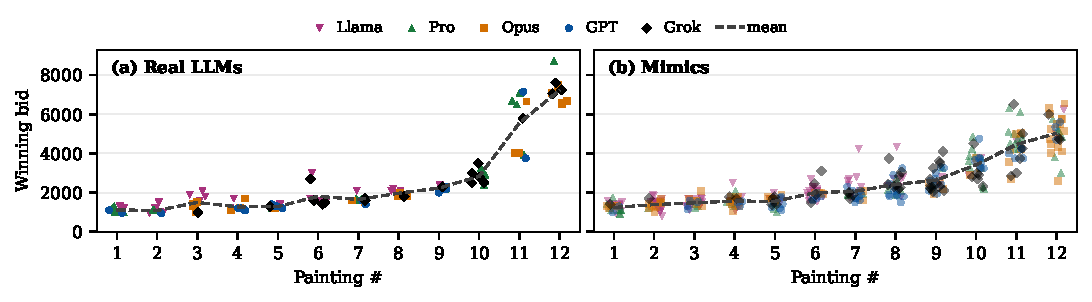
\includegraphics[width=0.9\textwidth]{auction_bids}
\caption{Winning bid per painting, by winning bidder: (a)~ten real-LLM and (b)~thirty mimic auctions (shared axes; dashed = per-painting mean). Both escalate at the end, but the mimics compress the spike ($3.8\times$ vs $2.4\times$ for the P11--P12 mean over P1--P10), missing the rare jump bids.}
\label{fig:auction_bids}
\end{figure*}

\subsubsection{Baseline Comparison}
Each baseline played 50 auctions against four rotating mimics (600 paintings each); with five bidders the fair share is $20\%$. Table~\ref{tab:math_results} reports win rates. Two findings stand out. First, performance is \emph{non-monotonic} in nominal sophistication: the Trivial min-bidder ($29.7\%$) substantially outperforms the principled Fair-Share budgeter, which wins \emph{no better than} the $20\%$ fair share ($19.5\%$, auction-level CI $[18.1,20.9]$, which includes $20\%$); the Trivial--Fair-Share gap is well outside both intervals. The mechanism is visible in the cap: early in the auction Fair-Share bids only up to $1.05\,B^i_t/n_t \approx \$875$, below the price at which early lots actually clear ($\sim$\$1{,}200; Fig.~\ref{fig:auction_bids}(a)), so it concedes the many cheap early paintings and hoards budget for the few expensive late lots. Since every painting counts equally, winning many cheap lots beats winning a few costly ones, and Trivial, bounded only by solvency, takes the early majority. Indeed, neither Fair-Share nor Reactive beats an ordinary LLM: in each of their batches Llama, the strongest model, wins a larger share of the lots it contests than the math policy (Fair-Share batch, $30.6\%$ vs.\ $19.5\%$; Reactive batch, $26.7\%$ vs.\ $23.8\%$), and the ordering repeats against the real LLMs ($29.2\%$ for Llama vs.\ $18.3\%$ and $25.0\%$). Their nominal sophistication buys nothing over the LLMs they aim to outclass. Among the math policies, RL has the highest mimic-field point estimate, but its interval overlaps those of Market-Clearing and Trivial (Table~\ref{tab:math_results}), so these three are statistically comparable rather than cleanly ordered.

Second, re-running every policy against the five real LLMs (5 auctions each) shows that the overall ordering transfers, but the top reshuffles. Fair-Share stays worst (below fair share), Reactive stays mid-pack, and Trivial, Market-Clearing, and RL still beat every LLM. Against the mimics RL has the highest point estimate (within overlapping intervals of Market-Clearing); against the real LLMs that nominal edge disappears, and the behavior-agnostic policies match or pass it: Trivial and Market-Clearing each reach $40\%$ while RL holds at $36.7\%$ (a two-painting margin, and all three intervals overlap heavily at $n=5$, so we read it as RL \emph{losing its lead} rather than being beaten). A plausible explanation, which we do not isolate directly, is that RL was trained against the mimics and fit surrogate-specific behavior that does not transfer, whereas Trivial (which models nothing) and Market-Clearing (which keys off opponent budgets, an observable, rather than a learned behavioral model) carry over cleanly, and the real LLMs concede contested lots even earlier than the mimics do. The mimics are thus reliable for \emph{comparing} fixed policies, but not for \emph{training} one to deploy against the real models.

\begin{table}[htbp]
\caption{Baseline win rates (percentages) with auction-level $95\%$ confidence intervals: against the mimic ensemble (50 auctions) and against the five real LLMs (5 auctions). Win rate is the mean of per-auction win fractions; the auction (not the painting) is the independent replicate, and intervals are $t$ intervals over auctions. Fair share with five bidders is $20\%$; bold marks the highest point estimate in each column (intervals may overlap). \emph{The vs-real column has only $n=5$: its intervals are approximate and overconfident (simulated coverage $\sim$75--90\% against a nominal $95\%$), and Reactive's $[25.0,25.0]$ reflects five identical auctions, not zero uncertainty. Treat that column as indicative.}}
\label{tab:math_results}
\centering
\begin{tabular}{lcc}
\hline
Policy & vs mimics (95\% CI) & vs real LLMs (95\% CI) \\
\hline
Trivial          & 29.7 [27.7, 31.6] & \textbf{40.0} [35.4, 44.6] \\
Fair-Share       & 19.5 [18.1, 20.9] & 18.3 [13.7, 23.0] \\
Reactive         & 23.8 [22.9, 24.8] & 25.0 [25.0, 25.0] \\
Market-Clearing  & 31.2 [29.3, 33.1] & \textbf{40.0} [35.4, 44.6] \\
RL               & \textbf{33.5} [31.9, 35.1] & 36.7 [31.0, 42.3] \\
\hline
\end{tabular}
\end{table}


\subsubsection{Synthesis}
The three results cohere into one account. The LLMs converge on a simple, one-dimensional strategy: a fair-share reservation price that governs when to drop out. That simplicity is what makes them \emph{distillable} (small networks reproduce their play at $V = 0.041$ and $88$--$93\%$ per-decision accuracy) and what makes them \emph{beatable} (a trivial minimum-bidder, a budget-aware heuristic, and a learned policy all exceed their share). The methodological caution we carry forward is the boundary of that distillability: a policy \emph{trained} against the mimics fails to transfer while fixed policies do, so behavioral mimics are faithful enough to \emph{compare} strategies but not to \emph{train} a deployable one.

% =====================================================================
% REVIEW LATER -- open auction scrutinies (statistical pass, 2026-06).
% Everything is backed up; nothing below is rendered. Decide, then delete.
%
% ALREADY APPLIED in this pass:
%  - Baseline table (tab:math_results) now carries auction-level t intervals
%    (unit = auction, n=50 / n=5), not painting-level. Verified against the
%    bootstrap; identical at n=50. vs-mimics CIs are trustworthy; vs-real (n=5)
%    are flagged overconfident in the caption.
%  - "Fair-Share below fair share" -> "no better than fair share"
%    (CI [18.1,20.9] includes 20%).
%  - "only Market-Clearing and RL clearly beat Trivial" -> softened: Trivial /
%    Market-Clearing / RL have OVERLAPPING CIs (statistically comparable).
%  - RL "learned to exploit the surrogate" -> "a plausible explanation, which we
%    do not isolate directly".
%  - milgrom-weber \cite key aligned to \bibitem{MilgromWeber}.
%  - Fidelity table (tab:mimic_fidelity) left on bootstrap CIs; deterministic
%    Welch t corroborates it (GPT [-1.3,+3.0]  Grok [-3.9,+0.6]  Llama [-0.9,+4.8]
%    Opus [-1.1,+4.5]  Pro [-6.3,+0.8]); all still include 0.
%
% NEEDS A DECISION (substantive -- not changed; may need a reframe or a run):
%  1. AGGRESSION vs INFORMATION confound. The win-rate order tracks cap
%     AGGRESSIVENESS (Trivial/MC/RL ~30-33%, overlapping CIs; Fair-Share/Reactive
%     clearly lower), not cleanly "information use". Prop 1 only proves MC is
%     >= Reactive in aggression, not that it uses opponent info *well*. The
%     "ladder of increasing information use" framing may be unsupported. Fix:
%     add an opponent-blind policy matched in aggression to MC to isolate the
%     information effect, OR reframe the ladder as a cap-aggression axis.
%  2. REWARD DEGENERACY. Money worthless + identical paintings => grabbing cheap
%     early lots is mechanically dominant, so "the aggressive policy wins" is
%     partly built into the reward. State as a scope limit or it reads as an
%     artifact, not a finding about LLMs.
%  3. MAGIC CONSTANTS (1.05 Fair-Share, 0.18 kappa, 1.75/1.15 eta). Confirm fixed
%     a priori, NOT tuned on eval data; add one sentence on provenance.
%  4. n=5 TRANSFER CIs are overconfident (coverage sim: t ~87%, percentile
%     bootstrap ~75%, both ~62% in the degenerate Reactive case). ASK: report a
%     Bayesian Beta-Binomial credible interval (won't degenerate), or keep
%     point+direction with the caveat? Real fix = more real-LLM auctions
%     (ask Prof. Zong re: API budget).
%  5. BEHAVIOR CHARACTERIZATION leans on chain-of-thought quotes, which are soft
%     evidence (CoT need not be faithful). Keep as qualitative color only;
%     consider trimming -- it is also the most perishable / least-novel part.
%  6. Pro is the worst-fit mimic (Delta -2.8, MAE 1.55) yet we claim "jumps don't
%     affect the win distribution" -- mild tension; fine to keep, note Pro is the
%     soft spot.
%  CONSISTENCY ASK: switch the fidelity table to the Welch t CIs above so the
%     whole section is seedless? (Currently fidelity=bootstrap, baseline=t.)
% =====================================================================
